\subsection{Differences with traditional ML}
\begin{frame}
  \frametitle{Traditional Machine Learning}
  \begin{itemize}
    \item Parametric model \( f_{\thetab}: \xb \rightarrow y \)
    \item Define a distance function \( d(\cdot, \cdot) \) and measure the
          distance (loss) from observed data
      \begin{equation}
        L(\thetab) = \sum_i^N d(f_{\thetab}(\xb^i), y^i)
      \end{equation}
    \item Search for the parameter set $\hat{\thetab}$ that reproduces the observed data best
      \begin{equation}
         \hat{\thetab} = \argmin_{\thetab} L(\thetab)
      \end{equation}
    \end{itemize}
    \noindent\makebox[\linewidth]{\rule{\paperwidth}{0.4pt}}
    We search for a \alert{single configuration (point-estimate) \( \hat{\thetab}\) }

\end{frame}

\begin{frame}
  \frametitle{Bayesian Formulation}
  \begin{itemize}
    \item On the modelling part:
      \begin{itemize}
        \item we need the \textcolor{blue}{joint distribution \(p(\xb,y,\thetab)\)}
        \item to replace the \textcolor{red}{parametric model \(f_{\thetab}: \xb \rightarrow y\)}
      \end{itemize}

    \item Training part:
      \begin{itemize}
        \item infer the \textcolor{blue}{posterior distribution \(p(\thetab|D)\)}
        \item to replace the optimal \textcolor{red}{point estimate \(\hat{\thetab} = \argmin_{\thetab} L(\thetab)\)}
      \end{itemize}

    \item Prediction part:
      \begin{itemize}
        \item infer the \textcolor{blue}{predictive distribution \(p(y|\xb,D)\)}
        \item to replace the \textcolor{red}{point-estimate prediction \(y=f_{\hat{\thetab}}(\xb)\)}
      \end{itemize}
    \end{itemize}
    \noindent\makebox[\linewidth]{\rule{\paperwidth}{0.4pt}}
    We replace point estimates \alert{with distributions (uncertainty quantification)}

\end{frame}

\begin{frame}
  \frametitle{Modelling part}
  \begin{itemize}
    \item joint distribution \( p(\xb, y, \thetab) = p(y|\xb,\thetab) p(\xb) p(\thetab) \)
    \item \( p(\thetab) \), our prior belief about the parameters of the model
    \item \( p(y|\xb, \thetab)\), the likelihood of the model
    \item joint distribution can be defined as a \alert{DAG}
  \end{itemize}

  \begin{figure}[!h]
  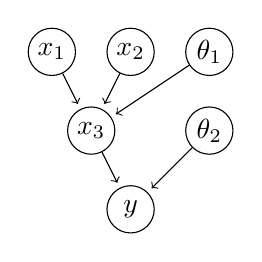
\begin{tikzpicture}[scale=.3]
  \node (x1) [draw, circle, xshift=0cm, minimum size=.6cm, inner sep=0pt]{$x_1$};
  \node (x2) [draw, circle, xshift=0cm, right of=x1, minimum size=.6cm, inner sep=0pt] {$x_2$};
  \node (th1) [draw, circle, xshift=0cm, right of=x2, minimum size=.6cm, inner sep=0pt] {$\theta_1$};
  \node (x3) [draw, circle, xshift=-.5cm, below of=x2, minimum size=.6cm, inner sep=0pt] {$x_3$};
  \node (th2) [draw, circle, xshift=1cm, below of=x2, minimum size=.6cm, inner sep=0pt] {$\theta_2$};
  \node (y) [draw, circle, xshift=.5cm, below of=x3, minimum size=.6cm, inner sep=0pt] {$y$};

  \draw [->, shorten >=2pt] (x1) -- (x3);
  \draw [->, shorten >=2pt] (x2) -- (x3);
  \draw [->, shorten >=2pt] (th1) -- (x3);
  \draw [->, shorten >=2pt] (x3) -- (y);
  \draw [->, shorten >=2pt] (th2) -- (y);
  \end{tikzpicture}
\end{figure}

\noindent\makebox[\linewidth]{\rule{\paperwidth}{0.4pt}}
\begin{itemize}
\item We need to model \alert{ \(p(\thetab) \text{ and } p(y|\xb, \thetab) \)}
\end{itemize}

\end{frame}


\begin{frame}
  \frametitle{Training part}
  \begin{itemize}
  \item We use Bayes law to infer the posterior distribution
    \begin{equation}
      p(\thetab|D) = \frac{p(D|\thetab)p(\thetab)}{p(D)} \propto \prod_i^N p(y^i|\xb^i, \thetab)p(\thetab)
    \end{equation}
    where $D = \{\xb^i, y^i\}_{i=\{1, ..., N\}}$, the observed data (training-set)
    \item In the extreme case where $p(\thetab|D) = \delta(\thetab - \hat{\thetab})$, we get a point-estimate is in traditional ML
    \end{itemize}

    \noindent\makebox[\linewidth]{\rule{\paperwidth}{0.4pt}}
    The `training process` leads to many possible models, each one with different probability (\alert{uncertainty about the model})

\end{frame}

\begin{frame}
  \frametitle{Inference part}
  \begin{itemize}
  \item We need to solve/approximate the predictive distribution $p(y|\xb, D) = \int_{\thetab} p(y|\xb,\thetab)p(\thetab|D) \partial \thetab$
  \item We consider the posterior $p(\thetab|D)$ as known (computed exactly or approximated)
  \item In the extreme case where
    $p(\thetab|D) = \delta(\thetab - \hat{\thetab})$, we get all the mass of the
    prediction $p(y|\xb, D) = p(y|\xb,\hat{\thetab})$ from a single model
  \end{itemize}

    \noindent\makebox[\linewidth]{\rule{\paperwidth}{0.4pt}}
  The `prediction process` gets one prediction per each
    plausible model (\alert{uncertainty about the model leads to uncertainty about the
    prediction})


\end{frame}

\subsection{Pros and Cons}
\begin{frame}
  \frametitle{Bayesian Formulation - Disadvantages}
  What we lose
  \begin{itemize}
  \item On the modelling part
    \begin{itemize}
    \item Time to think how the input features $x_i$ relate to each
      other i.e. building the DAG
    \end{itemize}
    \item On the training-prediction (inference) part
      \begin{itemize}
        \item Expressions difficult to approximate
        \item $p(\thetab|D)$ - how to compute the posterior distribution?
        \item $p(y|\xb,D) = \int_{\thetab} p(y|\xb, \thetab) p(\thetab|D)\partial \thetab$ - how to compute the predictive distribution?
      \end{itemize}
    \end{itemize}
\noindent\makebox[\linewidth]{\rule{\paperwidth}{0.4pt}}
Bayesian Formulation is \alert{difficult from both the mathematical and the computational point-of-view}
\end{frame}

\begin{frame}
  \frametitle{Bayesian Formulation - Advantages}
  What we get:
  \begin{itemize}
  \item On the modelling part
    \begin{itemize}
    \item Specify who the features relate to each other
    \item check \href{https://www.mbmlbook.com/}{Model-based Machine Learning} - a new approach for ML model building
    \end{itemize}
  \item On the inference part
    \begin{itemize}
    \item Uncertainty estimation! Why we need it?
    \item Most times the available data is not enough to reveal a single instance $\hat{\thetab}$
    \item Sometimes we want to predict on a new $\xb$ that is very
      different from the training set
    \end{itemize}
  \end{itemize}
\noindent\makebox[\linewidth]{\rule{\paperwidth}{0.4pt}}
\alert{Let's be wise enough and be uncertain about our predictions.}
\end{frame}


\begin{frame}

  \frametitle{Bayesian Formulation - Example}  \begin{itemize}
    \item In areas without training points our uncertainty is bigger
  \end{itemize}


  \begin{figure}[ht]
    \centering
    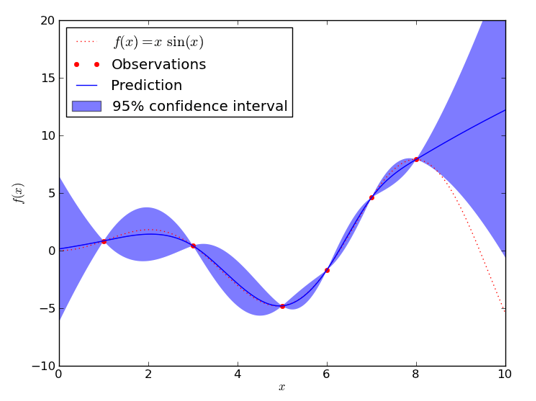
\includegraphics[scale=0.5]{./images/gp.png}
    \label{fig:bayesian_predictive}
  \end{figure}
\end{frame}
